\documentclass[12pt]{article}

\usepackage{fancyhdr}
\usepackage{amssymb}
\usepackage{amsthm}
\usepackage{amsfonts}
\usepackage{mathtools}
\usepackage{array}
\usepackage{systeme}
\usepackage{geometry}
\usepackage{enumitem}
\usepackage{ dsfont }
\usepackage{listings}
\usepackage{booktabs}
\usepackage{hyperref}
\usepackage{float}
\usepackage{tikz}
\usetikzlibrary{arrows,decorations.pathmorphing,backgrounds,positioning,fit}
\usetikzlibrary{automata, positioning}
\usetikzlibrary{calc}
\usepackage[utf8]{inputenc}
  \geometry{
    left = 2.5cm,
    right = 2.5cm,
    includeheadfoot, top = 1.5cm, bottom = 1.5cm,
    headsep = 1.3cm,
    footskip = 1.2cm
  }

% Inline fraction %
\newcommand*\rfrac[2]{{}^{#1}\!/_{#2}}
\newcommand{\lincom}[4]{\mathit{{#1}{\underline{#2}}}+\mathit{{#3}{\underline{#4}}}}
\newcommand*{\QEDA}{\hfill\ensuremath{\blacksquare}}
\newcommand*{\QEDB}{\hfill\ensuremath{\square}}
\newcommand{\MU}[1]{\mathit{\underline{#1}}}

\newcommand{\DS}{\displaystyle}
\newcommand{\bb}[1]{\mathbb{#1}}

% Absolute value: \abs{x} => |x|
\newcommand{\abs}[1]{\left|#1\right|}

% Function: \func{f}{X}{Y} => f : X -> Y
\newcommand{\func}[3]{#1 : #2 \rightarrow #3}
% Function to R: \func{f}{X} => f : X -> R
\newcommand{\functoR}[2]{#1 : #2 \rightarrow \mathbb{R}}
% Function to N: \func{f}{X} => f : X -> N
\newcommand{\functoN}[2]{#1 : #2 \rightarrow \mathbb{N}}
% Function from R to R: \func{f} => f : R -> R
\newcommand{\funcR}[1]{#1 : \mathbb{R} \rightarrow \mathbb{R}}

% Limits and convergence
\newcommand{\limn}{\lim_{n \to \infty}}
\newcommand{\limh}{\lim_{h \to 0}}
\newcommand{\limsupn}{\limsup_{n \to \infty}}
\newcommand{\liminfn}{\liminf_{n \to \infty}}
\newcommand{\limx}[1]{\lim_{x \to #1}}
\newcommand{\tounif}{\xrightarrow{unif.}}

% Sums and series
\newcommand{\sumn}[1]{\sum_{k=1}^n #1}
\newcommand{\series}[1]{\sum_{k=1}^\infty #1}
\newcommand{\seriec}[1]{\sum_{k=m}^n #1}
\newcommand{\pseries}[1]{\sum_{n=0}^\infty #1}

% Intervals
% Closed-closed interval [a,b]
\newcommand{\intcc}[1]{\left[#1\right]}
% Open-closed interval (a,b]
\newcommand{\intoc}[1]{\left(#1\right]}
% Closed-open interval [a,b)
\newcommand{\intco}[1]{\left[#1\right)}
% Open-open interval (a,b)
\newcommand{\intoo}[1]{\left(#1\right)}

% Sets
\newcommand{\N}{\mathbb{N}}
\newcommand{\Z}{\mathbb{Z}}
\newcommand{\Q}{\mathbb{Q}}
\newcommand{\R}{\mathbb{R}}
\newcommand{\e}{\varepsilon}

\lhead{Alexander Fischer, Camillo Malnati, Federico Pfahler, Aldo Gabriele di Rosa}
\chead{}
\rhead{}
\rfoot{\thepage}
\cfoot{}
\lfoot{\today}
\pagestyle{fancy}

\begin{document}
  \begin{center}
    \LARGE{\textbf{MindPollution}}
  \end{center}
  \section{Introduction}
  Bikes are an ecological way to move around cities. 
  There is a trend in cities to provide bikers preferential lanes and even bike-sharing services that aim to raise the usage of this transport over other transports methods, such as cars, motorbikes, but also public transports such as buses. 
  \emph{MindPollution} aims to collect and visualise pollution metrics inside cities by using small devices installed on public bikes. Bikes will not only provides excellent coverage over the city due to the freedom with which they can move in areas where other vehicles cannot, but they can also supply data from multiple bicycles and users at the same time.

  \subsection{Initial approach}
  Our initial idea was to create a user-independent device that would have been installed on the public-bikes, and that would have required no interactions with the users. The devices would have stored the information about the pollution directly on their memory, they would have then transferred the data to the database service only when a user reached a recognised official location for bike drop-off. Due to a broken GPS sensor and lack of time to get a new one, we had to rethink our approach and application. In fact, to create a map of the city, we still needed to have the position of the bike somehow.

  \subsection{Selected approach}
The broken GPS sensor implied the need to find new ways to get the position of the bike in the city. The first problem is that we couldn't rely on the bike since no requirements said that the public service would have provided this information to our application. The only way to have access to the position is to develop a mobile app that provides the user's locations and transmits the pollution information from the device directly to the phone. Now that the platform is user-dependant on regards of the device, we have decided to use the phone application to directly transfer data to the server, abandoning the idea of having data transmission stations. In the end, we also developed a web-application that visualises the collected data.
  \newpage
  \section{Implementation}
  In order to satisfy the requirements of our project we decided to go with an hybrid architecture with both an arduino board and a smartphone. This architecture is the results of not being able to find a properly working GPS board in time for the project deadline. We think this architecture will prove to be easier to scale with a large number of boards connected to the web server and database.

  Figure~\ref{fig:architecture} shows an overview of the architecture of our project, showing the main components.
  \begin{figure}[H]
    \centering
    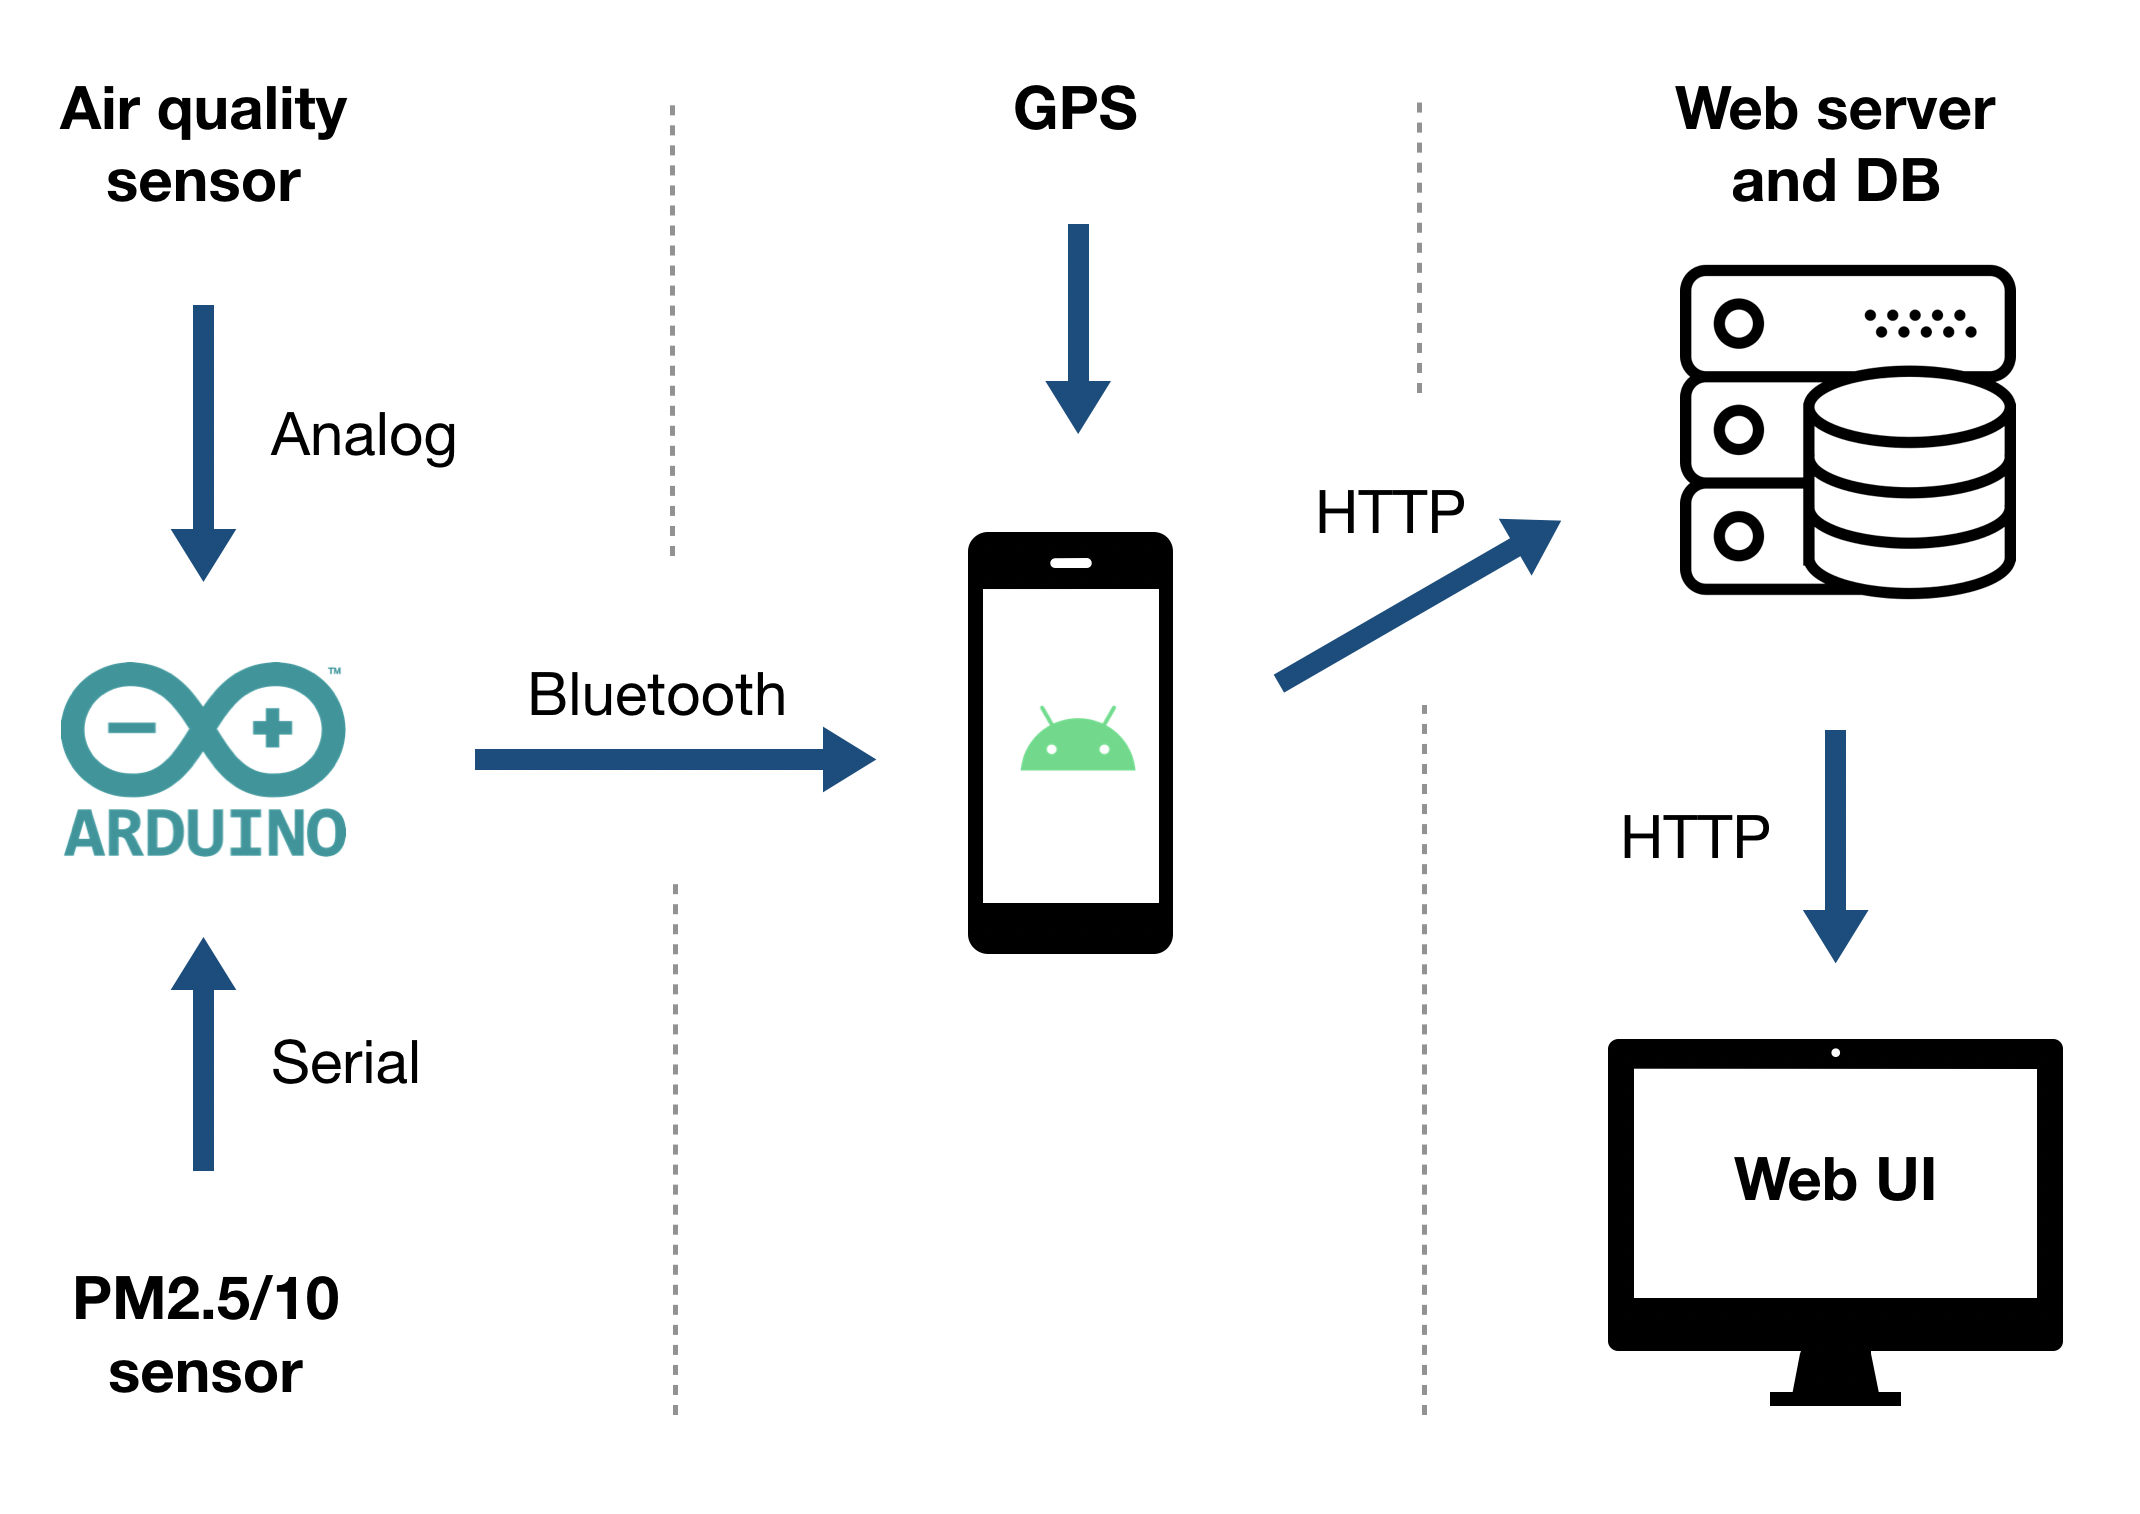
\includegraphics[width=0.7\textwidth]{images/architecture.png}
    \caption{An overview of the main components in our system.}
    \label{fig:architecture}
  \end{figure}

  Shown in \autoref{fig:project-photo} is a picture of the project components wired to the Arduino Nano board and how they are physically connected. These components are all powered by a battery pack (providing $6\ volts$) connected to a voltage regulator that decreases the voltage to $5\ volts$. While Arduino supports different power supply voltages, the two sensors that we used require that particular value.
  \begin{figure}[H]
    \centering
    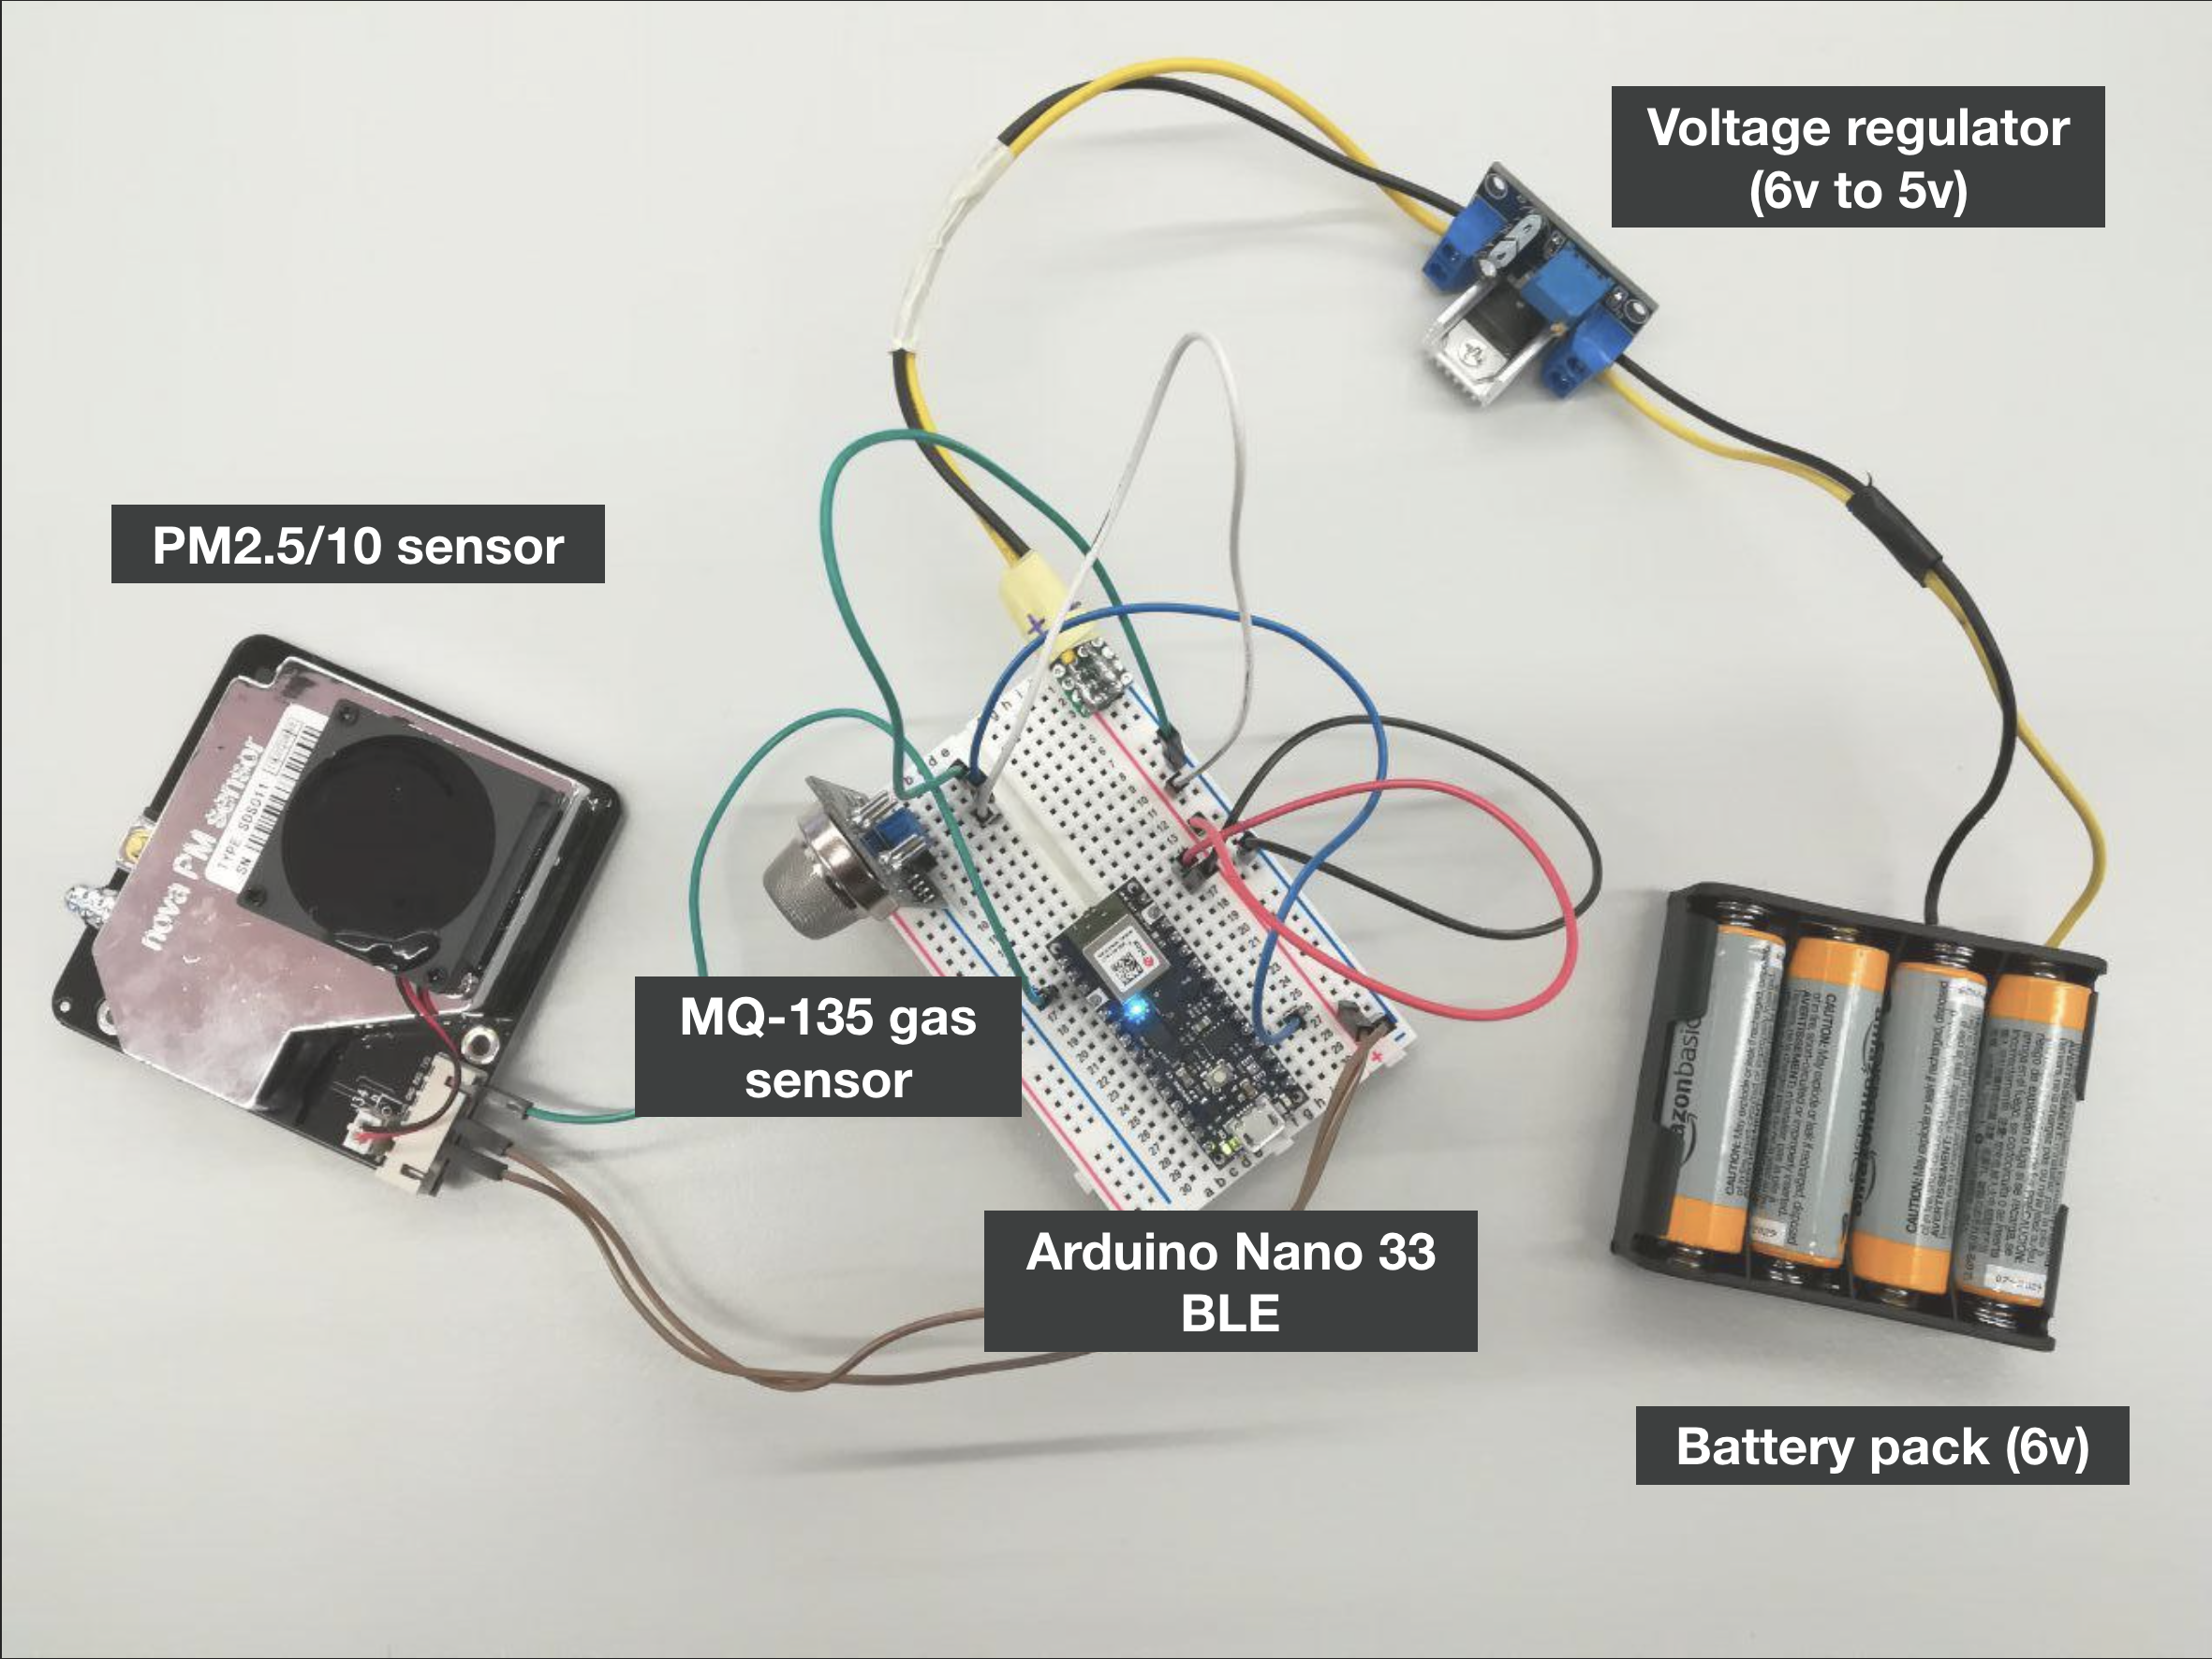
\includegraphics[width=0.7\textwidth]{images/project-all.png}
    \caption{A picture of the project components.}
    \label{fig:project-photo}
  \end{figure}
  
  \subsection{Sensors}
  To measure the air quality and pollutions levels we use two sensors that we connect directly to the Arduino board.
  \subsubsection{Air quality}
  \begin{figure}[H]
    \centering
    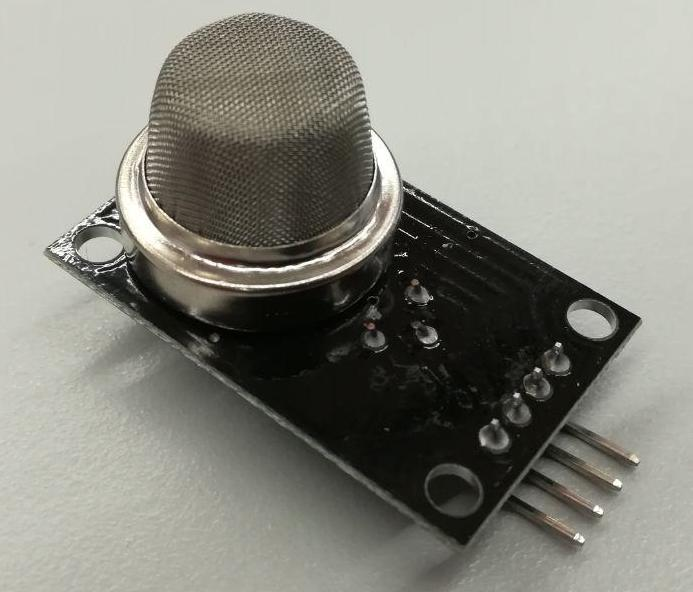
\includegraphics[width=0.5\textwidth]{images/mq-135.jpg}
    \caption{The MQ-135 gas sensor module}
    \label{fig:air-quality-photo}
  \end{figure}
  We measure the air quality by using a module, depicted in~\autoref{fig:air-quality-photo}, that includes a MQ-135 gas sensor (see datasheet\footnote{https://www.olimex.com/Products/Components/Sensors/Gas/SNS-MQ135/resources/SNS-MQ135.pdf}), which is sensitive to several pollutants including $NH_3$, $NO_x$, alcohol, benzene, smoke and $CO_2$.
  Its output is an aggregated level of \textit{air quality}, either as an analog voltage or as a digital output based on a threshold. An higher value implies that the density of the detected gases is higher, and therefore the air quality is worse.

  This module requires a supply voltage of $5\ volts$, and we connect its analog output to an analog input pin (i.e. $A0$) of our Arduino Nano board.

  \subsubsection{Particulate matter (PM2.5/PM10)}
  \begin{figure}[H]
    \centering
    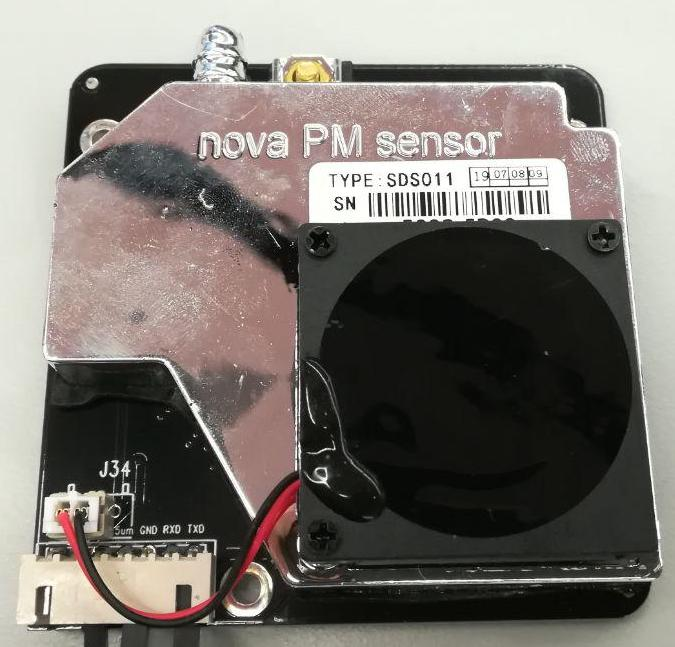
\includegraphics[width=0.5\textwidth]{images/pm-sensor.jpg}
    \caption{The Nova Fitness SDS011 PM2.5/PM10 sensor}
    \label{fig:pm-sensor-photo}
  \end{figure}
  Another sensor, shown in~\autoref{fig:pm-sensor-photo}, that we use to measure the pollution is the Nova Fitness SDS011 (see datasheet\footnote{https://cdn-reichelt.de/documents/datenblatt/X200/SDS011-DATASHEET.pdf}), which measures the density of particulate matter (i.e. PM2.5 and PM10) in the air. Its range of measured values is between $0$ and $999\mu g/m^3$.

  To output those values, the module has a serial interface based on the UART communication protocol, described in \autoref{tab:uart-protocol}, and the rate of transmission of the measurements is $1Hz$. We connected the output pin of this serial interface to the serial input pin of our Arduino Nano board. Furthermore, similarly to the air quality sensor, the module requires a supply voltage of $5\ volts$.

  \begin{table}[H]
    \centering
    \begin{tabular}{r | l | l}
      \# & Name & Content\\\toprule
      0 & Header & AA\\
      1 & Commander No. & C0\\
      2 & DATA 1 & PM2.5 Low Byte\\
      3 & DATA 2 & PM2.5 High Byte\\
      4 & DATA 3 & PM10 Low Byte\\
      5 & DATA 4 & PM10 High Byte\\
      6 & DATA 5 & ID Byte 1\\
      7 & DATA 6 & ID Byte 2\\
      8 & Checksum & Checksum\\
      9 & Tail & AB\\
    \end{tabular}
    \caption{The bytes sent over the serial interface}
    \label{tab:uart-protocol}
  \end{table}

  In order to extract the correct values of bot PM2.5 and PM10 the following formula should be applied to the content of \autoref{tab:uart-protocol}:

  \begin{itemize}
    \item PM2.5 value: PM2.5 ($\mu g/m^3$)  =  ((PM2.5  High  byte  *256)  +  PM2.5 low byte)/10
    \item PM10 value: PM10 ($\mu g/m^3$)  =  ((PM10  high  byte*256)  +  PM10  low byte)/10
    \item Checksum: Checksum=DATA1+DATA2+...+DATA6
  \end{itemize}

  \subsection{Arduino code}
  The Arduino code is quite easy to understand, it is divided into three main parts: Global variables, setup and main loop:

  \subsubsection{Global variables}
  We need this first part of the code to declare the global variables for the RGB light, the Bluetooth and the sensors. In particular we save the pins of the integrated RGB light on the Arduino Nano BLE board.

  We then create a buffer for the data we want to send on the Bluetooth as well as the Bluetooth service and characteristic. We defined the maximum length of the buffer sent via Bluetooth as 20 bytes long, that is the threshold we found was perfectly working for the transfer and it was big enough to hold all the data we needed to send in one transmission.
  The small dust particle sensor need also some variables to decode the protocol from the serial port.

  \subsubsection{setup()}
  As the name suggest this is the code setting up all we need for the project. First the serial port transmission, then the Bluetooth service to which we assign a specific name and then we start advertising.

  \subsubsection{loop()}
  This is the main part of the program that is also divided in two main branch. The device is connected to the RGB light turns green and the program reed from the small dust particle serial the data that is coming. There is a specific protocol (see~\autoref{tab:uart-protocol}) that we need to decode in order to extract the data. When one correct reading is completed the code takes a reading also on the air quality sensor and sends the data via Bluetooth to the connected smartphone application. The data is sent with a specific sequence as follows: \verb|<PM10>,<PM2.5>,<AIR_QUALITY>;|.

  If the device is not connected instead, a blinking blue light will start and the Arduino boards will start advertising again until a device get connected to it.
    


  \subsection{Android application}
  The goal of the Android application is to act as a \textit{gateway} between the Arduino board that collects pollution data from sensors and the web application that stores and visualizes the aggregated data. While forwarding pollution measurements, it also adds the current location coordinates obtained from the phone's GPS sensor.

  The application runs on a mobile phone (in our demo a Huawei P10 lite running Android 8.0) that is connected via Bluetooth to the Arduino Nano 33 BLE board, as well as with an active GSM connection.
  Its source code is based on an example application, \verb|BluetoothLeGatt|\footnote{Also on Github: https://github.com/android/connectivity-samples/tree/master/BluetoothLeGatt}, which is bundled with the official Android SDK, that allows to scan for Bluetooth Low Energy devices and connect to them. 

  What we added to that code was to, on every message received from the Arduino board, retrieve the location coordinates (code is adapted from a blog post\footnote{https://medium.com/@ssaurel/getting-gps-location-on-android-with-fused-location-provider-api-1001eb549089}) and send that data together with the pollution information to a web server as a JSON object by performing a POST request. 
  
  An example of such JSON object is shown in Figure~\ref{lst:json-packet}. On the other hand, the message sent from the board is structured as follows: \verb|123,12,5;|. It contains the measurements from the air quality sensor, as well as the two measured values from the PM2.5/10 sensor.

  \begin{figure}[H]
    \centering
    \begin{verbatim}{
  "createdAt": "2019-12-13T09:22:49.824Z",
  "lat": 46.0037,
  "long": 8.9511 ,
  "bikeId" : "00002add-0000-1000-8000-00805f9b34fb",
  "pm10": 5,
  "pm25": 12,
  "airQuality": 123
}\end{verbatim}
  \caption{An example JSON object containing the pollution measurements and location}\label{lst:json-packet}
  \end{figure}
  The application user interface, shown in~\autoref{fig:app-scan-list}, is comprised of two main views: the device list and the device information.
  The first view allows the user to scan for nearby Bluetooth Low-energy devices and shows them as a list. We modified the existing code to only visualize devices with the name \verb|AIR_QUALITY|, so that, for demonstration purposes, only our Arduino board would be shown.

  \begin{figure}[H]
    \centering
    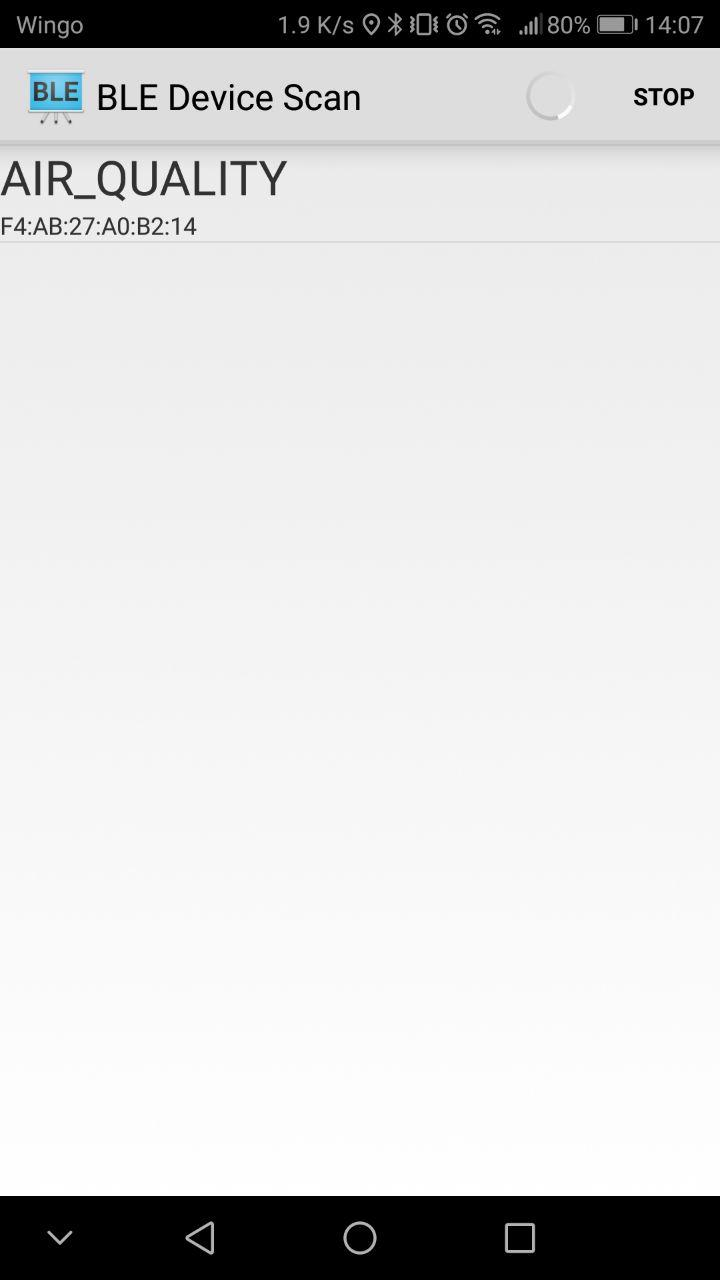
\includegraphics[width=0.3\textwidth]{images/android1.jpg}
    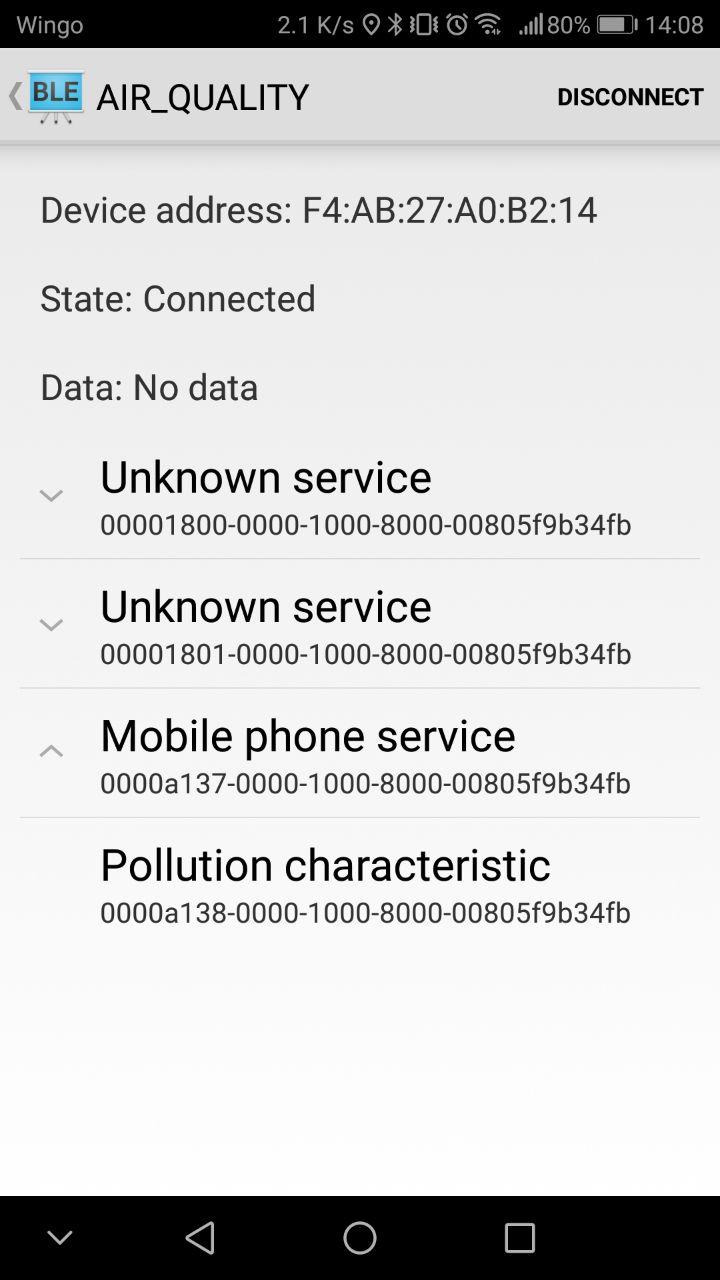
\includegraphics[width=0.3\textwidth]{images/android2.jpg}
    \caption{The two main views of the application: device list (left), device information (right)}
    \label{fig:app-scan-list}
  \end{figure}

  When selecting a device, the other view is shown, visualizing more information related to that device and allowing the user to connect to it. The information shown includes the device address, the connection status, the last packet of data received as well as a list of the BLE services and characteristics that the device advertises. By tapping on a characteristic (in our case: \textit{``Pollution characteristic''}), notifications for it are enabled. The application will then listen for the data received from the connected device, process it and forward it to the remote server, as described previously.
  This view was already present in the example code, and what we added was the code for listening to and processing the data notifications from the Arduino board.

  \subsection{Web application}
  The goal of the web application is to visualise the data collected from the devices. The frontend uses Leflet 
  \newpage
  \section{Conclusions}
  The idea of using public bikes services to collect pollution data has been proven to be useful, especially since this service is widely used in cities. The device responsible for collecting data can be easily extended by using other sensors in addition to the ones that have been selected for this project, also providing different types of information from the current ones. Regarding the visualisation, it can provide detailed information about the quality of the air, giving insights about the areas that are more polluted. Regarding future work, sensors still have a significant impact on battery consumption, creating the need for improving the sampling of the data to save energy.  Right now, due to the missing GPS sensor, the tool is user-dependent. This can lead to problems since to collect data; users will need to download an application. This can be resolved by inserting the GPS in the device and by implementing the approach explained in Section 1.1.   

\end{document}
